\documentclass{99-Styles/CCAP}

\input 99-Styles/GetPackages
\input 99-Styles/Definitions

\usepackage{afterpage}

\begin{document}

\input 00-Top-matter/00-Top-matter

\makeatletter
%\linenumbers
%\modulolinenumbers[5]

\begin{center}
  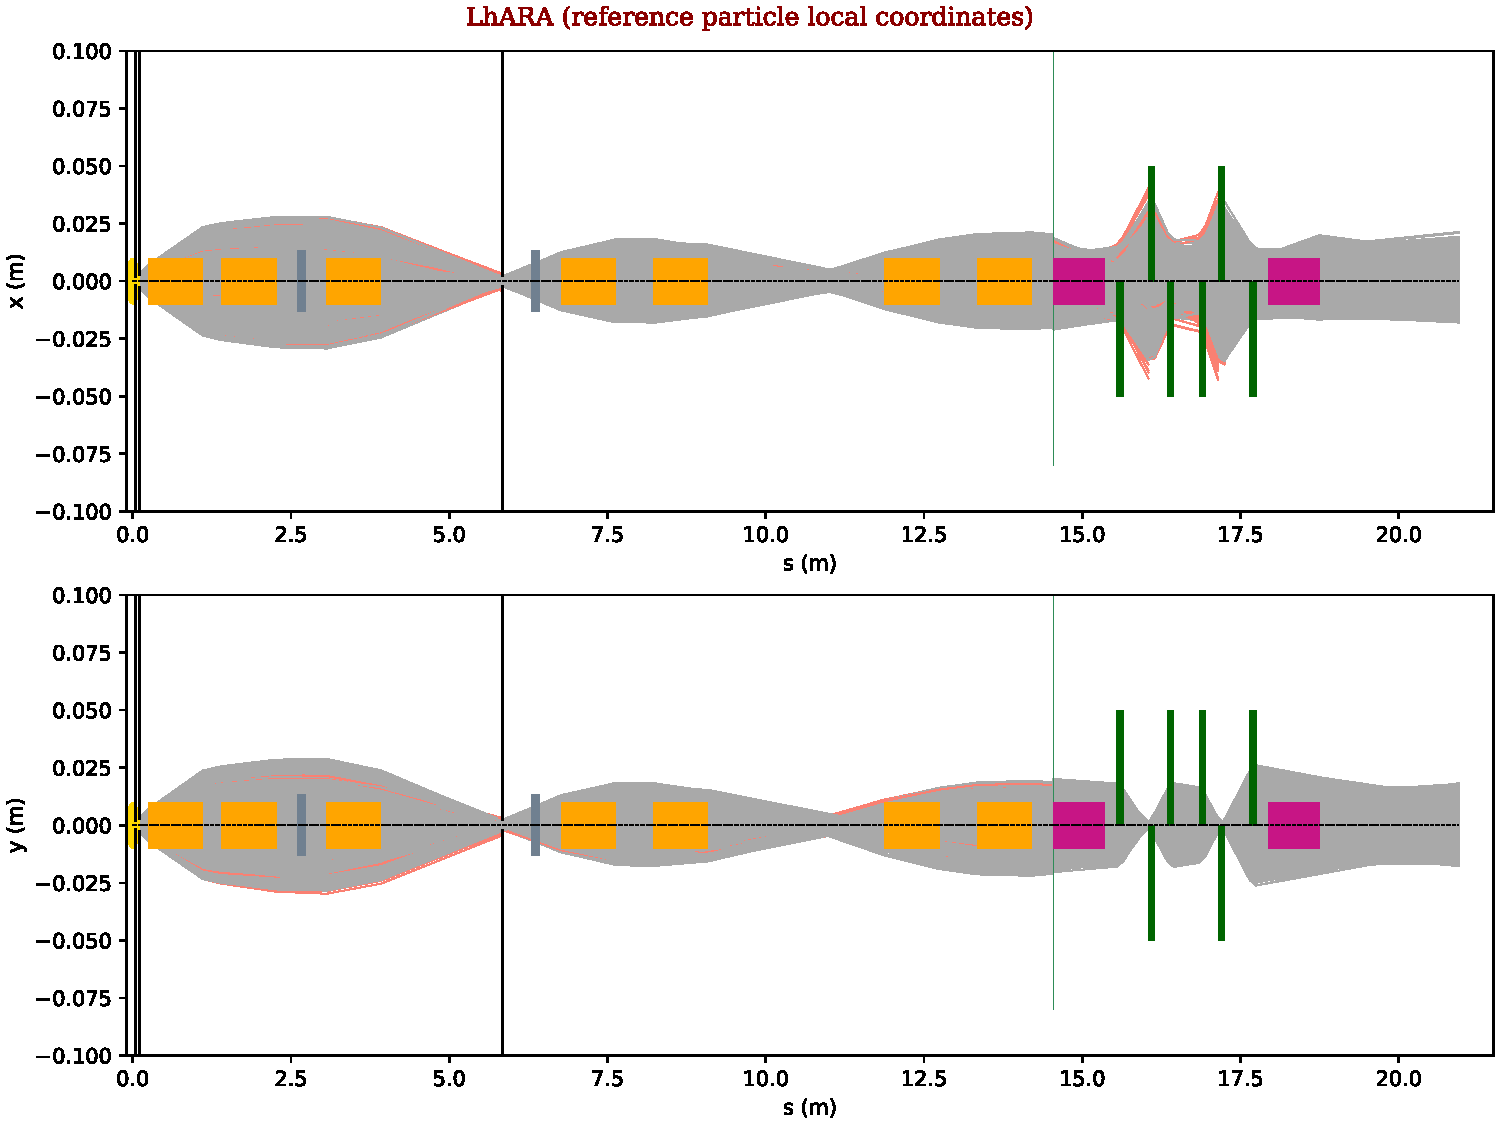
\includegraphics[width=0.75\textwidth]{00-Top-matter/Figures/LhARA-RPLC.pdf}
  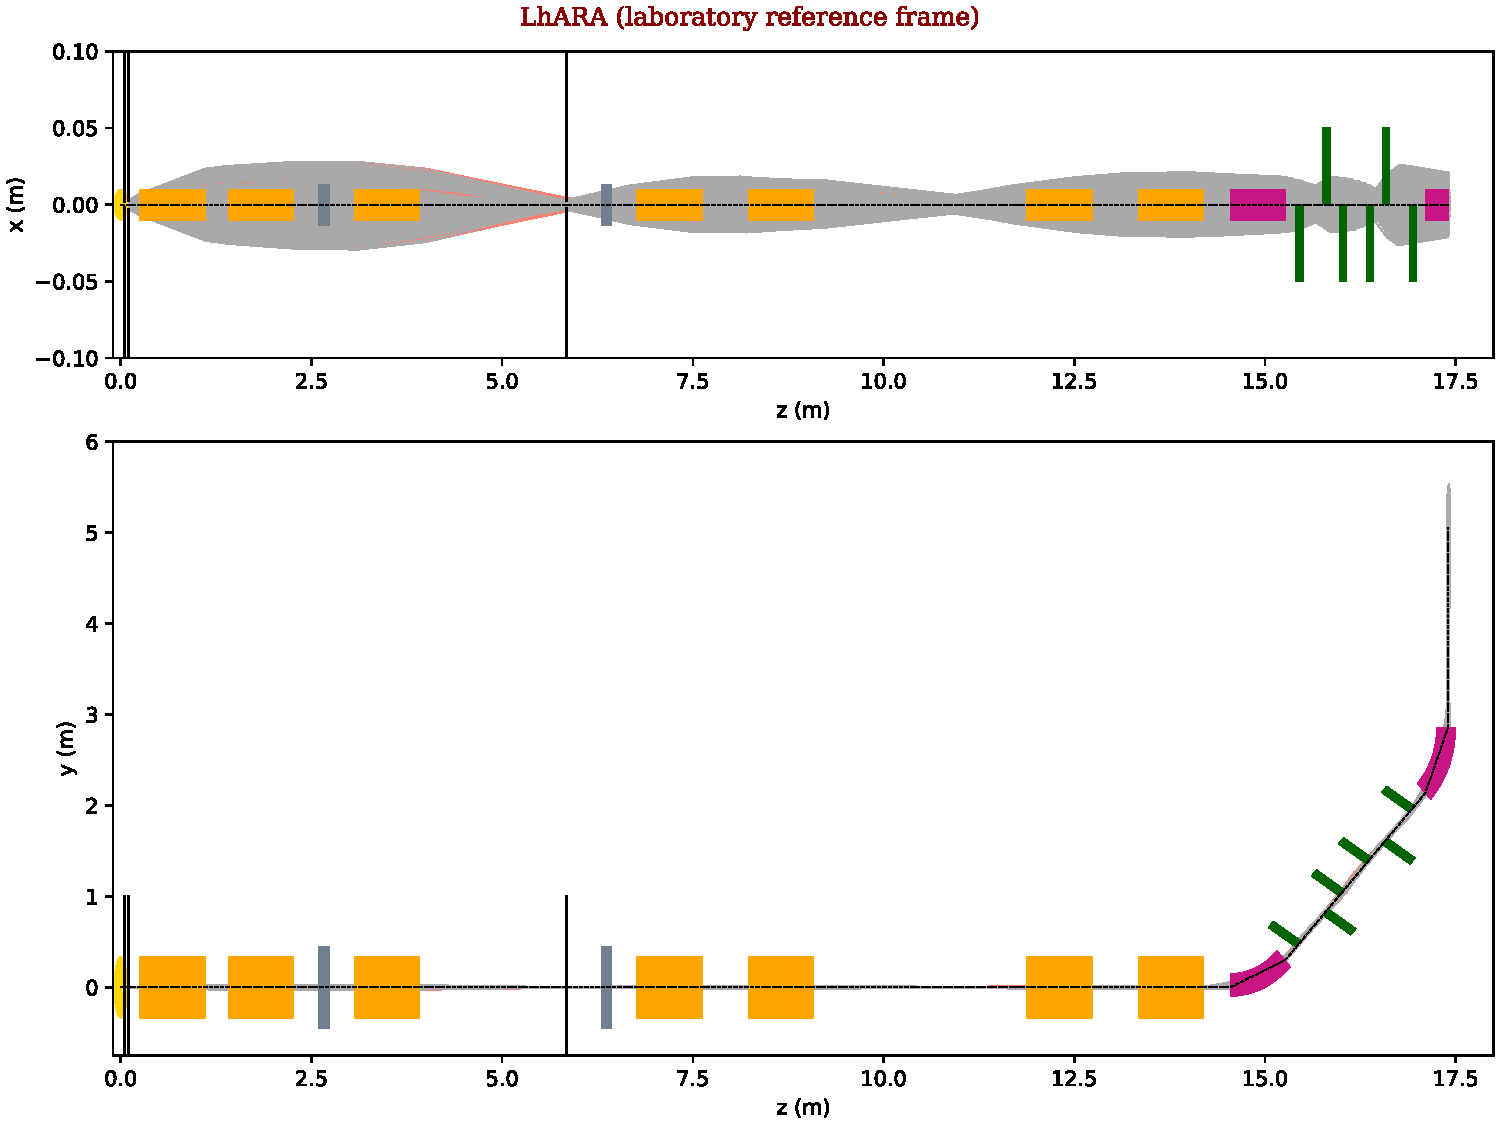
\includegraphics[width=0.75\textwidth]{00-Top-matter/Figures/LhARA-lab.pdf}
\end{center}

\clearpage

\thispagestyle{empty}
%\setcounter{tocdepth}{3}
\tableofcontents

\clearpage

\parindent 10pt
\pagenumbering{arabic}                   
\setcounter{page}{1}

\pagestyle{plain}

\vskip 1.0cm
\input 01-Intro/01-Intro
\input 02-CoordinateSystems/02-CoordinateSystems
\input 03-PhaseTraceSpace/03-PhaseTraceSpace
\input 04-TransferMatrices/04-TransferMatrices
\input 05-Source/05-Source
\input 06-BLspecScrpts/06-BLspecScrpts

\addcontentsline{toc}{section}{Acknowledgements}
\input 91-Acknowledgements/91-Acknowledgements

\clearpage
\addcontentsline{toc}{section}{References}
\bibliographystyle{99-Styles/utcaps}
\bibliography{Concatenated-bibliography}

\clearpage
\appendix
\input A1-MCD/A1-MCD
\input A2-SetupRun/A2-SetupRun

\end{document}

